\section{Les informations à être visibles}

Dans la fiche d'incident, les informations suivantes doivent être visibles :

\begin{itemize}
    \item La date courante (assignée automatique) de chaque changement de statut
        (mise en triage, ouverture, escalades, etc.) ;
    \item Un identifiant unique automatiquement associé à l'incident,
        permettant la gestion a travers une infrastructure et le référencement
        entre incidents en relation ;
    \item La catégorie de l'incident (avoir des sous-catégories, 
        de préférence), permettant de filtrer et d'assigner l'incident directement
        au service concerné ;
    \item L'appareil (système d'exploitation, navigateur, nom de la machine, ...) ;
    \item La version si applicable ;
    \item Les étapes pour reproduire (si applicable) ;
    \item La priorité de l'incident ;
    \item Le niveau d'impacte de l'incident ;
    \item Le ou les services impactés
        (machine locale, un service donné, un système donné, ...) ;
    \item Le status de l'incident (voir la section \ref{S:status}) ;
    \item Personne(s) assigné-e-s ;
    \item Le nom de l'utilisateur et ses informations de contact
        (téléphone, courriel, bureau, etc.) ;
    \item Problèmes connus/ résolus en relation.
\end{itemize}

\begin{figure}[H]
    \centering
    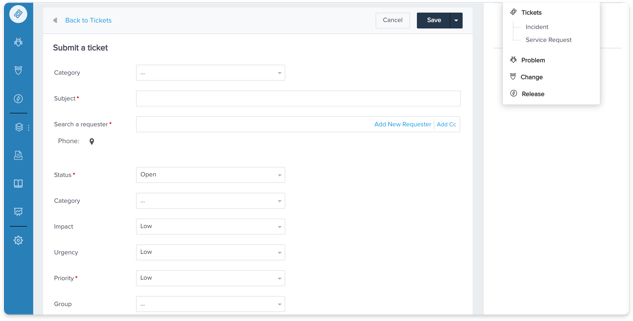
\includegraphics[width=.864\linewidth]
    {assets/empower-employees-with-self-service-5a1a79af.png}
    \caption{Exemple d'interface regroupant les différentes informations requises}
\end{figure}
